\documentclass{article}

\usepackage{url} 

\usepackage{pdfpages}
\usepackage{lastpage}
\usepackage{fancyhdr}
\usepackage{ngerman}
\usepackage{listings}

\usepackage{tabularx}
\usepackage{floatrow}
\usepackage[tableposition=top]{caption}
\floatsetup[table]{capposition=top}

\usepackage{amsmath, amssymb}

\usepackage[utf8]{inputenc}


\usepackage[numbib]{tocbibind}



\newcommand\twodigits[1]{%
   \ifnum#1<10 0#1\else #1\fi
}



\lhead{Interferometer}
\rhead{13. November 2020\\T. Maier, J. Winkler}
%\cfoot{\twodigits{\thepage}~/ \pageref{LastPage}}
\cfoot{{\thepage}~/ \pageref{LastPage}}

\newcommand{\W}{\text{W}}
\newcommand{\V}{\text{V}}
\newcommand{\A}{\text{A}}


\newcommand{\mini}{\operatorname{min}}


\begin{document}

\parindent0cm

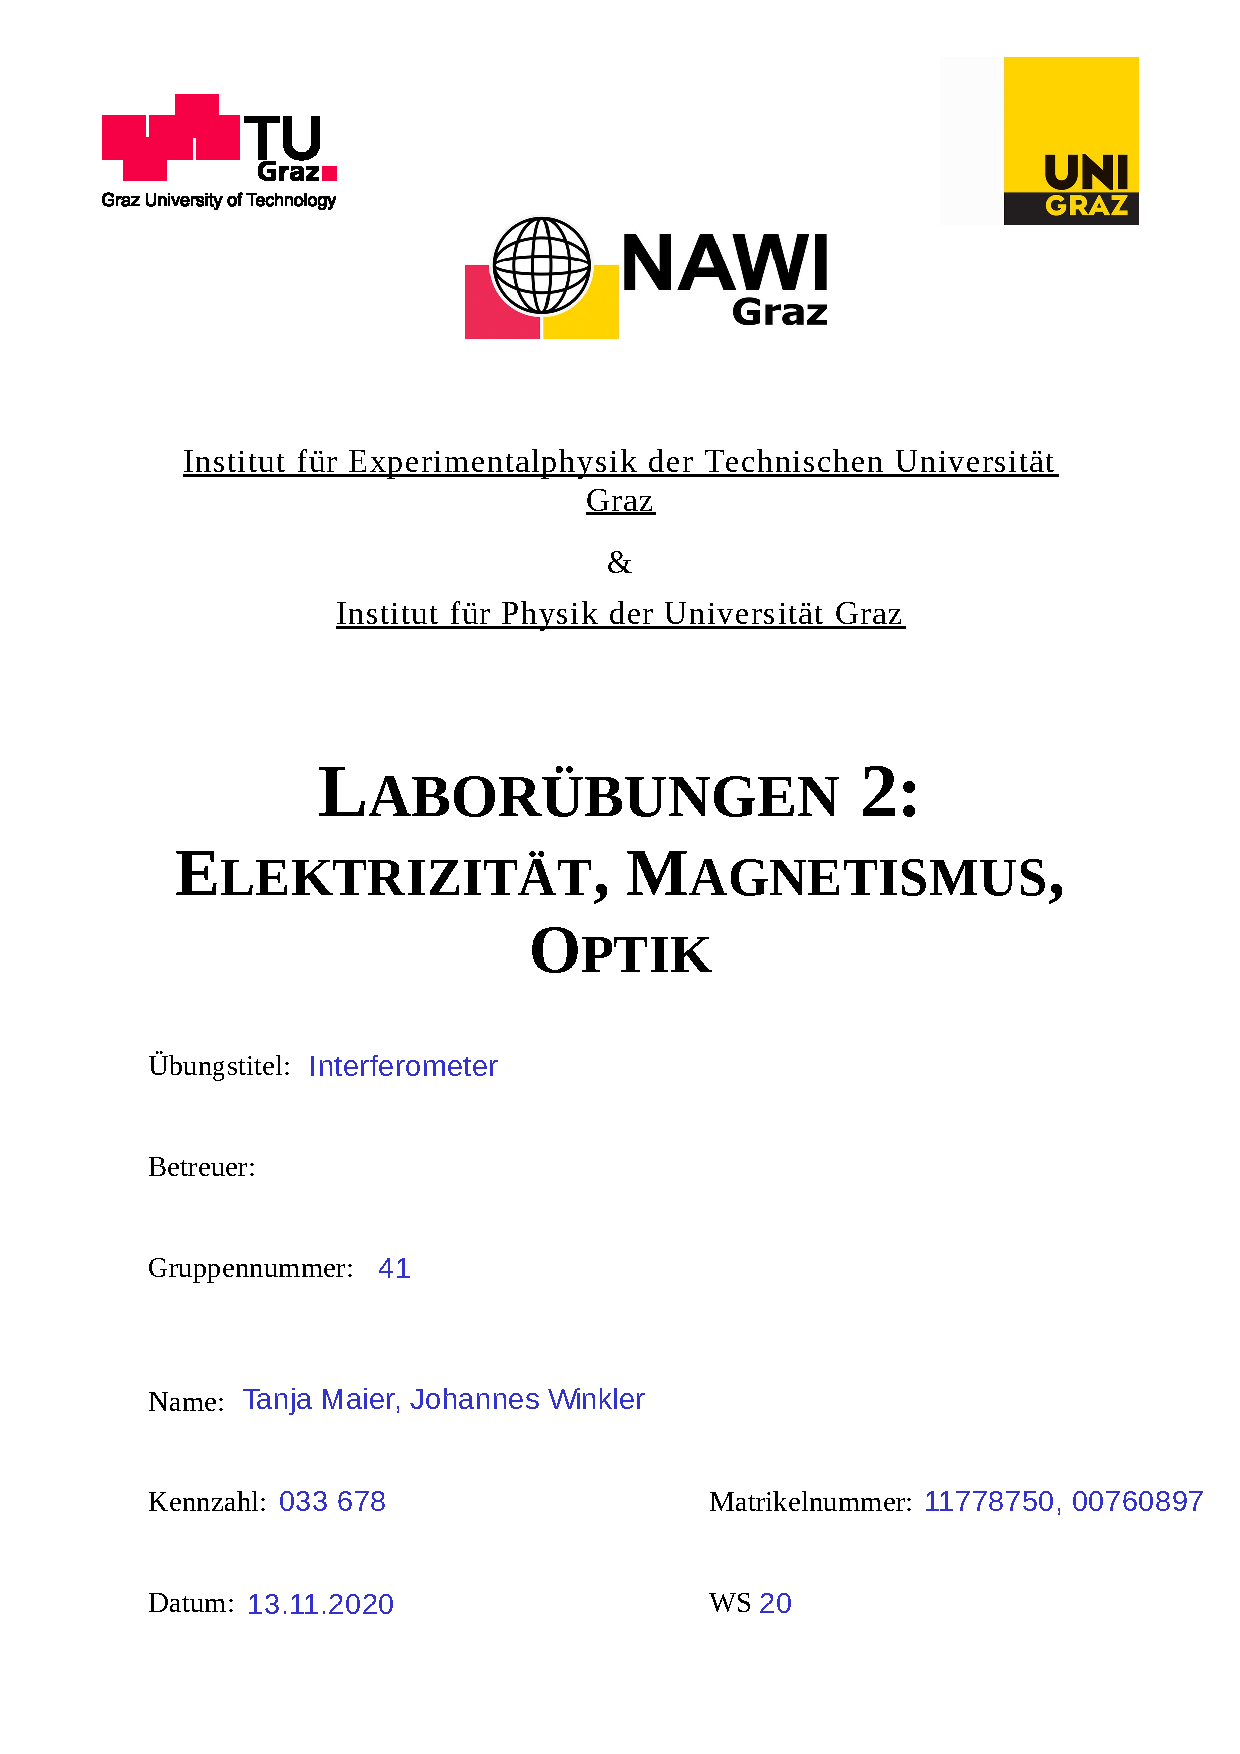
\includepdf{Deckblatt.pdf}


\pagestyle{fancy}

\section{Aufgabenstellung}

\begin{enumerate}
\item Demonstration und Erklärung des Einflusses der Größe einer Lichtquelle auf das Interferenzmuster eines Doppelspaltes.
\item Demonstration und Erklärung des Einflusses der spektralen Breite des Lichtes einer räumlich kohärenten Lichtquelle auf das Interferenzmuster eines Doppelspaltes.
\item Bestimmung der Dicke einer Kunststoffschicht mit dem Doppelspalt Interferenzmuster.
\item Bestimmung der Größe der Lichtquelle, bei der für Doppelspalten mit unterschiedlichem Spaltabstand das Licht noch räumlich kohärent ist.
\end{enumerate}



\section{Voraussetzungen und Grundlagen}

Grundlage dieses Versuchs bietet die Wellennatur des Lichts. Licht kann als elektromagnetische Welle im sichtbaren Spektralbereich gesehen werden. Das von einer Quelle ausgesendete Licht kann dann mit einem Doppelspalt in mehrere Teilwellen aufgespalten werden. Wenn dieses Teilwellen dann wieder aufeinandertreffen (z.B. durch Totalreflexion an einem Spiegel), so kommt es je nach Gang- bzw. Zeitunterschied entweder zur Auslöschung (destruktive Interferenz) oder Verstärkung (konstruktive Interferenz) der wieder vereinigten Welle. Wichtig ist dabei, dass die Welle sowohl zeitlich als auch räumlich kohärent (Amplitude und Phase sind also an jedem Punkt und zu jeder Zeit eindeutig definiert) ist. Dann gilt
\begin{align}
\Delta s = d \cdot \sin \theta_n = n\cdot \lambda \qquad n\in \mathbb{N}_0
\end{align}
wobei der Gangunterschied der beiden Teilwellen $n$-ter Ordnung, $d$ der Abstand der Spalten, $\theta_n$ der $n$-te Beugungswinkel, n die Ordnung des Interferenzmaximums und $\lambda$ die Wellenlänge ist.

Die Interferenzmaxima werden außerdem mit einer Sammellinse erfasst und abgebildet. Für den Abstand $b_n$ zwischen $0$-tem und $n$-tem Maximum gilt folgender Zusammenhang 
\begin{align}
b_n = f_2 \cdot tan\left( \operatorname{arcsin}\left(\frac{n\cdot\lambda}{d}\right)\right), \qquad n\in\mathbb{N}_0
\end{align}
wobei $f_2$ die Brennweite der Sammellinse nach dem Doppelspalt ist. Außerdem kann man noch den Kontrast $K$ des Inferenzmusters bestimmen, welcher von der jeweiligen Intensität der Lichtquelle abhängt.
\begin{align}
K = \frac{I_\text{max}-I_\text{min}}{I_\text{max}+I_\text{min}}
\end{align}
wobei $I$ die Intensität, $f_1$ die Brennweite der Sammellinse vor dem Doppelspalt und $\omega$ der Radius der Lichtquelle ist. Außerdem wird bei diesem Experiment auch eine Probe mit Polyacrylat verwendet, welche eine zusätzliche Phasenverschiebung am Doppelspalt bewirkt. Diese Phasenverschiebung kann beschrieben werden durch
\begin{align}
\Delta s_0 = \Delta s + t\cdot (n_1-n_2) = d\cdot\sin(\theta)\cdot t\cdot (n_1-n_2)
\end{align}
wobei $t$ die Dicke der Probe, $n_1$ der Brechungsindex der Probe und $n_2$ der Brechungsindex der Umgebung (hier: Luft, also n2 = 1) ist.


%\begin{figure}[H]
%\caption{Transformator}
%\label{fig:transformator}
%{\centering
%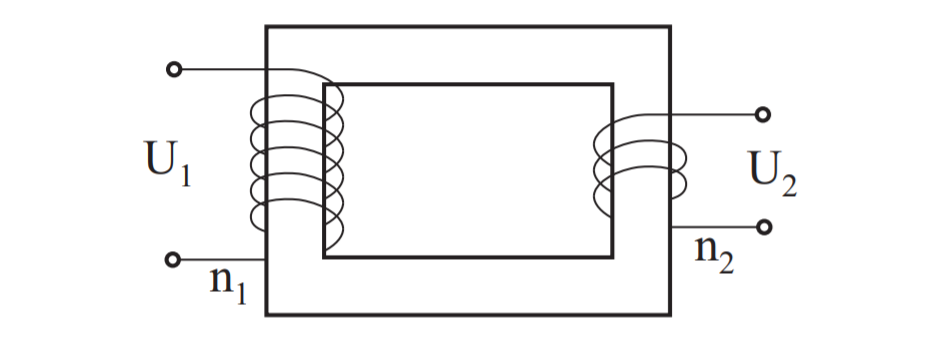
\includegraphics[scale=0.4]{transformator.png}
%~
%}
%\end{figure}





\section{Geräteliste}

\begin{table}[H]
\caption{Liste der verwendeten Geräte}

~

\begin{tabular}{l|p{3cm}p{3cm}llll}
Abk. & Bezeichnung  & Typ & Gerätenummer & Unsicherheit \\
\hline
S & Spaltblende \\
\hline
L1 & Sammellinse 1 & $f_1 = 300~$mm & & $\Delta f_1 = 0.5~$mm \\
\hline
L2 & Sammellinse 2 & $f_2 = 150~$mm & & $\Delta f_2 = 0.5~$mm \\
\hline
L3 & Sammellinse 3 & $f_3 = 40~$mm & & $\Delta f_3 = 0.5~$mm \\
\hline
L4 & Sammellinse 4 & $f_4 = 30~$mm & & $\Delta f_4 = 0.5~$mm \\
\hline
DS & Doppelspalt \\
\hline





B & Lochblenden und Irisblende & $d_1=2~$mm ~ ~ ~ ~ $d_2=3~$mm   ~~~~~~~~~~~~ $d_3=6~$mm & &  $\Delta d = 0.1~$mm \\
\hline
F & Filterrad für LEDs & \\
\hline
K & Kamera
\end{tabular}

\end{table}



\section{Beschreibung der Versuchsanordnung}








\section{Versuchsdurchführung und Messwerte}

\subsection{Teil 1}
Für diesen Versuch wurde monochromatisches Licht verwendet. Dann wurde der $633~$nm Bandpassfilter in den Strahlengang gedreht und der mittlere Doppelspalt in den Strahlengang geschoben.

Dann wurden 6 geeignete Größen der Lichtquelle gewählt, um den Verlauf des Kontrastes gemäß im Bereich $0 < 2\cdot w < 1.5 \cdot \lambda\cdot f_1 / d$ darstellen zu können. Dafür wurde zunächst die Spaltbreite des Kontrast-Minimums bestimmt. Beim Wert 0 der Mikrometerschraube war der Spalt jedoch noch nicht ganz geschlossen, sodass mit einer negativen Spaltbreite begonnen wurde, um den Spalt auch ganz geschlossen zu halten.
Für die gewählten Größen der Lichtquelle wurde jeweils ein Foto des Beugungsmusters aufgenommen (Abbildung xy).


\subsection{Teil 2}

Beim zweiten Versuch wurde die Spaltblende so eingestellt, dass das Licht mit 0.43 mm Spaltabstand räumlich gut kohärent ist. Danach wurde ein Beugungsbild mit dem 633 nm Bandpassfilter, mit dem Langpassfilter und ohne Filter aufgenommen (Abbildung xy).


\subsection{Teil 3}

Hier wurde der vorderste Doppelspalt mit 0.43 mm Spaltabstand verwendet und alle Filter aus dem Strahlengang gedreht. Danach wurde die mit Polyacrylat überzogene Probe in den Strahlengang eingebracht und mit einer Justierschraube verschoben, sodass die Polyacrylat-Schicht nur einen der beiden Spalte abdeckt. Dann wurde das Bild des verschobenen und ein Bild des nicht verschobenen Beugungsmusters, sowie ein Bild ohne Polyacrylat als Referenzwert aufgenommen (Abbildung xy).

\subsection{Teil 4}

In diesem Versuch wurde wieder monochromatisches Licht mit einem Bandpass von 633 nm verwendet. Für jeden der drei Doppelspalte wurde dann ein Bild aufgenommen (Abbildung xy) und durch Beobachtung des Beugungsbildes die minimale Spaltbreite für das erste Minimum vom Kontrast des Beugungsmusters bestimmt.
Die Messpunkte wurden in Tabelle xy notiert.


\section{Auswertung}








\section{Zusammenfassung und Diskussion}




%\newpage 
%\appendix
%\section{Python Skript}



\definecolor{commentgreen}{RGB}{2,112,10}
\definecolor{eminence}{RGB}{108,48,130}
\definecolor{weborange}{RGB}{255,165,0}
\definecolor{frenchplum}{RGB}{129,20,83}

\lstdefinelanguage{python}{
    morekeywords={def, for, range, abs, return},
    otherkeywords={<-,->, |>, \%\{, \}, \{, \, (, )},
    sensitive=true,
    morecomment=[l]{\#},
    morecomment=[n]{/*}{*/},
    morecomment=[s][\color{purple}]{:}{\ },
    morestring=[s][\color{orange}]"",
    commentstyle=\color{commentgreen},
    keywordstyle=\color{eminence},
    stringstyle=\color{red},
	basicstyle=\ttfamily,
	breaklines,
	showstringspaces=false,
	frame=tb
}
%\lstinputlisting[language=Python,captionpos=b, label=lst:test,caption={Python Skript}]{generate_numbers.py}

%\lstinputlisting[language=Python,captionpos=b, label=lst:test,caption={Bessel Auswertung}]{generate_numbers_bessel.py}


%\lstinputlisting[language=Python,captionpos=b, label=lst:test,caption={Zerstreuungslinse Auswertung}]{generate_numbers_zerstreuungslinse.py}


\begin{thebibliography}{9}
\bibitem{quelle1} \url{https://www.youtube.com/watch?v=oFJCEGcwUiQ}, 07.11.2020, 00:15 Uhr
\bibitem{quelle2} \url{https://www.spektrum.de/lexikon/physik/abbesche-theorie/13}, 07.11.2020, 00:17 Uhr
\bibitem{quelle3} \url{https://www.univie.ac.at/mikroskopie/1_grundlagen/optik/opt_instrumente/7_abbe.htm}, 07.11.2020, 00:24 Uhr
\bibitem{quelle4} \url{https://physik.cosmos-indirekt.de/Physik-Schule/Rayleigh-Kriterium}, 07.11.2020, 00:26 Uhr
\bibitem{quelle5} \url{https://www.youtube.com/watch?v=PZaUY45ce8k}, 07.11.2020, 00:27 Uhr
\bibitem{quelle6} Unterlagen aus Moodle, H. Ditlbacher, bereitgestellt von der KF Universität Graz
\end{thebibliography}


\end{document}
